\section{Umsetzung}

\textauthor{\vJB,}{\vLB,}{\vHS}

Das vorliegende Kapitel befasst sich mit der Umsetzung des Versuchssystems und des Demosystems.
Dazu wird zunächst eine Technologieentscheidung durchgeführt.
In einem weiteren Schritt wird die systematische Umsetzung der beiden Systeme dargestellt.

\subsection{Technologieentscheidung}

\textauthor{\vJB,}{\vLB,}{\vHS}

Die Technologieentscheidung unterteilt sich ebenfalls in eine eigenständige Entscheidung für das Versuchssystem, sowie das Demosystem.
Durch die Abhängigkeit der beiden Systeme, bezieht sich die Technologieentscheidung des Demosystems auf die Entscheidung des Versuchssystems.

\subsubsection{Versuchssystem}\label{sec:TechnologieVersuchssystem}

\textauthor{\vJB,}{\vLB}{}

Aus der Konzeption in Kapitel~\ref{sec:Konzeption} gehen verschiedene Anforderungen an die Technologie hervor.
Durch die Verwendung von neuronalen Netzen werden die verfügbaren Technologien bzw. Programmiersprachen bereits eingeschränkt.
Um weitere Technologieentscheidungen zu treffen, muss zunächst eine Programmiersprache ausgewählt werden.
Da in einer Umfrage unter Machine-Learning-Entwicklern und Data Scientists 57~\% Python als Programmiersprache nutzen und 33~\% diese sogar priorisieren, wird für dieses Projekt Python als Programmiersprache festgelegt \autocite[vgl. ][S. 16]{vision_mobile_state_2017}.
In einer allgemeinen Umfrage zu verwendeten Programmiersprachen liegt Python mit 49,2~\% auf Platz drei \autocite[vgl.][]{yepis_2023_2023}.
Das bedeutet, dass knapp die Hälfte der befragten Entwickler unter anderem Python verwenden, somit ist eine ausreichende Verbreitung gewährleistet.
Die Verbreitung ist vor allem deshalb ein wichtiger Aspekt, da es durch eine hohe Verbreitung ein großes Eco-System mit vielen quelloffenen Ressourcen und bereits durchgeführten Projekten gibt.

Um Machine-Learning mit Python zu betreiben, gibt es mehrere Bibliotheken zur Auswahl.
Die drei bekanntesten Open-Source-Bibliotheken sind dabei \gqq{TensorFlow}, \gqq{PyTorch} und \gqq{SciKit-Lern} \autocite[vgl.][]{msv_tensorflow_2020}.

Diese Bibliotheken sind sich relativ ähnlich.
Vorteile einer Bibliothek bringen automatisch auch Nachteile, die sich somit gegenseitig aufheben.

Für diese Studienarbeit wird TensorFlow genutzt, da es laut der \gqq{Stack Overflow Developer Survey 2022} eine größere Nutzerbasis hat \autocite[vgl.][]{stack_overflow_stack_2022}.
Zudem spricht für diese Entscheidung auch die Tatsache, dass die Entwickler dieser Studienarbeit bereits Vorkenntnisse in TensorFlow haben.

Zusätzlich wird das Modul \gqq{Keras} verwendet, welches eine entwicklerfreundliche High-Level-Schnittstelle für TensorFlow ist und somit eine einfachere Entwicklung ermöglicht \autocite[vgl.][]{noauthor_keras_2023}.

\subsubsection{Demosystem}

\textauthor{\vHS}{}{}

Für die Technologieentscheidung muss zunächst zwischen den zwei Komponenten Client und Server unterscheiden werden.
Da für beide Teile unterschiedliche Anforderungen erfüllt werden müssen, erfolgt die Technologieentscheidung separat.
Außerdem findet eine Festlegung des verwendeten Protokolls für die Schnittstellenkommunikation statt.

\paragraph{Client}
Die grundlegende Anforderung an den Client ist die Umsetzung als Webapplikation.
Daraus leiten sich in erster Linie vier verschiedene Programmiersprachen ab: JavaScript/Type\-Script, Python, PHP und Ruby.

Für eine weitergehende Einschränkung ist der vorausgesetzte Funktionsumfang relevant.
Dieser ist sehr gering, da lediglich Input-Elemente für die Angabe eines zu authentifizierenden Sprechers, sowie zur Auswahl einer zu verwendeten Datei bereitgestellt werden müssen.
Außerdem muss eine Verbindung zu einem Back-End (Server) aufgebaut werden können.

Da diese Anforderungen durch alle vier Kandidaten erfüllt werden, muss die Entscheidung durch andere Kriterien erfolgen.
Hierbei spielen vor allem zwei Aspekte eine Rolle.
Eine Umfrage von Stack Overflow aus dem Jahr 2020 zeigt, dass JavaScript die beliebteste Programmiersprache von professionellen Entwickler ist.
Moderne Frameworks wie ReactJS und Angular haben die klassische Webprogrammierung in PHP über die letzten Jahre abgelöst \autocite[vgl.][]{stack_overflow_stack_2020}.

Da es sich außerdem um ein Demosystem handelt, welches lediglich die Ergebnisse dieser Arbeit präsentieren soll und somit nicht in einem produktiven Umfeld betrieben wird, spielt die Technologieentscheidung nur eine untergeordnete Rolle.
Die Kompetenzen des Entwicklerteams liegen vor allem im Bereich der React Programmierung mit JavaScript beziehungsweise TypeScript.

Zusammenfassend fällt die Technologieentscheidung für die Client-Implementierung somit auf das JavaScript Framework ReactJS in Kombination mit TypeScript.
TypeScript ermöglicht dabei gegenüber JavaScript die Verwendung von Datentypen, wodurch Datentypfehler im Rahmen der Implementierung vermieden werden können.

\paragraph{Schnittstelle}
Im Web-Umfeld spielt das \ac{HTTP} eine besondere Rolle.
Dabei handelt es sich um ein zustandsloses Protokoll zur Übertragung von Daten auf der Anwendungsschicht.
Ein Anwendungsfall ist dabei die Anfrage von Webseiten im Browser über die URL.
Dazu wird eine sogenannte \ac{HTTP}-GET Anfrage an den Zielserver gesendet, welcher anschließend mit der angeforderten Ressource antwortet.

Nach demselben Prinzip kann das HTTP Protokoll ebenfalls dazu verwendet werden, eine Kommunikation zwischen Client und Server zu ermöglichen.
Die zu übergebenden Variablen des Clients an den Server können dabei innerhalb der URL des GET-Requests übertragen werden.
Gleichzeitig können die Ergebnisse des Servers beispielsweise im JSON-Format an den Client zurückgesendet werden.

Da das HTTP Protokoll somit alle benötigten Anforderungen erfüllt, kommt es für die Schnittstellenkommunikation zum Einsatz.

\paragraph{Server}
Für den Authentifizierungsprozess implementiert der Server denselben Ablauf wie das Versuchssystem.
Um eine doppelte Entwicklung zu vermeiden, entsteht somit eine Abhängigkeit zwischen der Technologieentscheidung des Versuchssystems und des Servers.
Aus der Technologieentscheidung des Versuchssystems in Kapitel~\ref{sec:TechnologieVersuchssystem} geht die Programmiersprache Python hervor.
Somit sollte zunächst geprüft werden, ob die Anforderungen des Servers in der Sprache Python umsetzbar sind.

Neben dem Authentifizierungsprozess spielt ausschließlich die Schnittstellenkommunikation zwischen Client und Server eine Rolle für die Technologieentscheidung des Servers.
Da als Kommunikationsprotokoll HTTP eingesetzt wird, muss also eine Bibliothek gefunden werden, die die Verwendung dieses Protokolls in Python ermöglicht.
Hierzu kann Flask verwendet werden.

Bei Flask handelt es sich um ein Web Framework, welches eine Bereitstellung von \ac{API} Endpunkten, die über das \ac{HTTP} Protokoll abrufbar sind, ermöglicht.

Somit können alle Anforderungen an die Serverapplikation mittels der Programmiersprache Python umgesetzt werden.
Dazu können die bereits entwickelten Komponenten für den Authentifizierungsprozess aus dem Versuchssystem übernommen werden.

\subsection{Versuchssystem}\label{sec:UmsetzungVersuchssystem}

\textauthor{\vJB,}{\vLB}{}

Die Umsetzung des Versuchssystems unterteilt sich in vier Unterkapitel.
Analog zu der Konzeption des Versuchssystems in Kapitel~\ref{sec:KonzeptVersuchssystem}, wird zunächst auf die Generierung der Feature-Kombinationen eingegangen.
Anschließend wird ein Datensatz ausgewählt und für die Verwendung in diesem System vorbereitet.
Daraufhin wird die Umsetzung der Audio-Vorverarbeitung sowie der Feature-Extraktion genau beschrieben.
Abgeschlossen wird das Kapitel mit der Umsetzung der Klassifikation und Evaluierung.

\subsubsection{Feature-Kombination}

\textauthor{\vLB}{}{}

Wie bereits in Kapitel~\ref{sec:FeatureKombination} erwähnt, müssen zuerst die verschiedenen Konfigurationen erzeugt werden.
Hierzu werden die vorher definierten Werte in einer JSON-Datei erfasst und durch ein eigenes Kombinierungs-Skript alle möglichen Konfiguration mit einer ID erzeugt.

Die Konfigurationswerte für die Kombinierung sind im Listing~\ref{lst-configs} dargestellt.

\begin{lstlisting}[language=Python,caption=Konfigurationsmöglichkeiten,label=lst-configs]
Configs = {
    "amount_of_frames": [10000, 15000],
    "size_of_frame": [400, 600],
    "LPC": {
        "order": [13, 20],
        "weight": [0, 1]
    },
    "MFCC": {
        "order": [13, 20],
        "weight": [0, 1]
    },
    "LPCC": {
        "order": [13, 20],
        "weight": [0, 1]
    },
    "delta_MFCC": {
        "order": [13],
        "weight": [0, 1]
    }
}
\end{lstlisting}

Der \texttt{weight} Parameter gibt lediglich an, ob in dieser Konfiguration dieses Feature verwendet werden soll oder nicht, um verschiedene Kombinationen zu erreichen.
So gibt es auch manche Kombinationen, die beispielsweise nur \ac{MFCC}-Merkmale in der Analyse berücksichtigen.
Hierbei muss beachtet werden, dass durch die Kombination auch Konfigurationen entstehen, in welchen nichts berechnet werden muss.
Diese werden manuell entfernt.
Die anderen Variablen wie \texttt{order} und dessen Werte wurden bereits in Kapitel~\ref{sec:FeatureKombination} erklärt.

\subsubsection{Datensatz}

\textauthor{\vLB}{}{}

Für die Evaluierung der Stimmmerkmale wird ein geeigneter Datensatz benötigt.
Hierzu wurde nach einer Internetrecherche auf der Plattform \gqq{Kaggle} ein entsprechender Datensatz gefunden, der die Anforderung aus Kapitel~\ref{sec:KonzeptDatensatz} erfüllt \autocite[vgl.][]{jain_speaker_2019}. 
Der Originaldatensatz enthält Audiodaten zu 50 Sprechern mit mindestens 60 Minuten Aufzeichnung pro Sprecher in mehreren kompressionslosen WAV Dateien.

In einem ersten Schritt müssen die Daten manuell aufbereitet werden.
Der Originaldatensatz lässt sich in zwei Teile teilen, während der erste Teil aus YouTube Videos besteht, sind im zweiten Teil Aufnahmen von englischen Hörbüchern enthalten.
Da die Aufnahmequalität der Hörbücher deutlich besser ist, werden nur diese Datensätze weiterverwendet.
In einem Folgeschritt werden die einzelnen Dateien der Datensätze zu einer Datei zusammengefügt und genauer betrachtet.
Hierbei können längere Pausen und Abweichungen der Datensätze, wie z.B. mehrere Sprecher oder eine andere Sprache identifiziert werden.
Diese Pausen werden entfernt und die betroffenen Datensätze aus dem Datensatz entfernt.
Dadurch bleiben 25 geeignete Datensätze übrig, aus diesen werden unter dem Aspekt des Geschlechts 20 Datensätze ausgewählt, sodass neun weibliche und elf männliche Sprecher im finalen Datensatz sind, da nur neun weibliche Datensätze geeignet sind.
Abschließend wird für jeden Sprecher eine Audiodatei zum Trainieren des neuronalen Netzes mit acht Minuten und zur Evaluation neun Sequenzen mit jeweils 15 Sekunden erstellt.
Das Testmaterial ist nicht im Trainingsmaterial enthalten.

\subsubsection{Vorverarbeitung und Feature-Extraktion}\label{section:umsetzung-versuch-vorverarbeitung}

\textauthor{\vJB}{}{}

Um eine effektive Verarbeitung eines Audiosignals zu ermöglichen, muss zunächst eine Vorverarbeitung des Signals erfolgen (s. Kapitel~\ref{sec:preprocessing}).
Hierfür wird der Audio-Clip mittels der Bibliothek \gqq{Librosa} geladen.
Anschließend folgt der erste Schritt der Vorverarbeitung, das Entfernen von stillen Passagen.
Dafür wird ein selbst entwickelter Algorithmus verwendet, der erkennt, wenn sich die Amplitude des Audiosignals über einen gewissen Zeitraum unterhalb eines definierten Schwellwerts befindet.

\begin{lstlisting}[language=Python,caption=Remove Silence,label=lst-remove-silence]
for i, amp in enumerate(y):
if abs(amp) < threshold:
    counter_below_threshold += 1
else:
    if counter_below_threshold > pause_length_in_ms:
        for index in range(i-counter_below_threshold+keep_at_start_and_end, i-keep_at_start_and_end):
            indices_to_remove.append(index)
    counter_below_threshold = 0
\end{lstlisting}

Nach dem Entfernen der Pausen wird das Hintergrundrauschen entfernt.
Dafür wird ein externer Algorithmus von Tim Sainburg verwendet.
Dieser basiert auf dem Vorgehen des bekannten Ton-Verarbeitungsprogramm \gqq{Audacity}.
Zusammengefasst transformiert der Algorithmus mithilfe von \ac{FFT} das Audio-Signal zunächst in den Frequenzraum.
Hier werden dann die Störfrequenzen über Schwellwertverfahren lokalisiert und mittels Filter eliminiert.
Anschließend wird das Signal wieder zurücktransformiert \autocite[][]{sainburg_timsainbnoisereduce_2019}.

Die abschließende Unterteilung des Audiosignals in Frames, sowie das Windowing der Frames findet mit Hilfe von \texttt{numpy}-Operationen in den Funktionen \texttt{create\_\-frames()} und \texttt{window\_\-frames()} statt.
Die passende Fensterfunktion wird dabei ebenfalls durch die \texttt{numpy}-Bibliothek bereitgestellt.
Bei dem Aufteilen in Frames wird eine Überlappung von 50 \% gewählt.

Für das Extrahieren der Merkmale aus dem Audiosignal wird ein Ansatz gewählt, der eine einfache Erweiterung des Programms um verschiedene andere Verfahren ermöglicht.
Dazu wird das Designmuster Strategie in abgewandelter Form verwendet, wobei zunächst ein Interface für die Berechnungsverfahren erstellt werden muss.
Dieses definiert die Funktion \texttt{calculate\_features()}, welche in den abgeleiteten Klassen implementiert wird.
Für die eigentlichen Berechnungen der Koeffizienten wird wieder die Signal-Verarbeitungs-Bibliothek Librosa verwendet.
Beispielhaft für die Berechnung von \ac{MFCC} sieht man in Listing~\ref{lst-MFCCExtractor}, wie unkompliziert sich die Bibliothek Librosa verwenden lässt.
Allerdings müssen viele Parameter, wie zum Beispiel die Länge des zu verwendenden FFT-Fensters (\texttt{n\_fft}) gefüllt bzw. geändert werden.
Diese Werte ergeben sich aus den von uns ausgewählten Parameter (beschrieben in~\ref{sec:FeatureKombination}) und den Anweisungen in der offiziellen Dokumentation der Librosa-Bibliothek \autocite[vgl. ][]{librosa_development_team_librosa_2023}.

\begin{lstlisting}[language=Python,caption=Klasse zur Extraktion von MFCC-Merkmalen,label=lst-MFCCExtractor]
class MFCCExtractor(ExtractorInterface):

@staticmethod
def calculate_mfcc(frame, sr, order):
    mfcc = librosa.feature.mfcc(y=frame, sr=sr, n_mfcc=order, n_fft=1024, hop_length=512)
    mfcc_of_frame = np.mean(mfcc.T, axis=0)
    return mfcc_of_frame

def calculate_features(self, frames, sr, order, multiprocessing=False):
    if multiprocessing:
        with Pool(8) as p: # run function on 8 cores
            mfccs = p.starmap(self.calculate_mfcc, [(frame, sr, order) for frame in frames])
        return mfccs
    else:
        mfccs = []
        for frame in frames:
            mfccs.append(self.calculate_mfcc(frame, sr, order))
        return mfccs
\end{lstlisting}

Da für die Versuchsreihe sehr viele zeitaufwändige Berechnungen laufen müssen, ist das Extrahieren der Merkmale mit Multiprocessing implementiert.
Hierfür wird die Python-interne Bibliothek \gqq{mutliprocessing} genutzt, um die Berechnung auf mehrere Kerne zu verteilen.

% librosa load 
% remove silence 
% noice_reduce#

% berechnung der Merkmale für Trainings- und Testdaten --> benötigt für Traditionellen Authentifizierungsprozess

\subsubsection{Klassifikation und Evaluierung}

\textauthor{\vJB,}{\vLB}{}

In dem Kapitel~\ref{sec:KonzeptKlassifikation} wurden neuronale Netze als Klassifikationsmodell gewählt, um die zuvor berechneten Merkmale zu evaluieren.
Hierbei werden zuerst neuronale Netze mit den berechneten Trainingsdaten trainiert.
Die Netze bestehen aus drei Hidden-Layer mit jeweils 128, 64 und 32 Neuronen.
Dieser absteigende Aufbau stellt sich bei Versuchen als geeignete Lösung heraus.

Wie bereits im Konzept dargestellt müssen mehrere neuronale Netze trainiert werden, in diesem Fall werden für jede Konfiguration drei neuronale Netze erstellt.

\begin{lstlisting}[language=Python,caption=Erstellen und Trainieren eines neuronalen Netzes,label=lst-nn]
# create model
tf.keras.backend.clear_session()
model = tf.keras.models.Sequential([
    tf.keras.layers.Flatten(input_shape=[input_layer_neurons]),
    *hidden_layer, # 128, 64, 32
    tf.keras.layers.Dense(output_layer_neurons, activation=tf.nn.softmax),
])
model.compile(optimizer=tf.optimizers.Adam(), loss='sparse_categorical_crossentropy', metrics=['accuracy'])

# train model
model.fit(X, y, epochs=epochs)
\end{lstlisting}

Nach dem Training erfolgt die Evaluation der neuronalen Netze, hierzu wird der tatsächliche Authentifizierungsprozess nachgebildet.
Die berechneten Testdaten werden auf die neuronalen Netze angewandt, das neuronale Netz klassifiziert also die Daten, indem es die Features jedes Frames einem der 20 Sprecher zuordnet.
Diese Klassifizierung wird durch die Tensorflow-Methode \texttt{model.predict()} realisiert, wie das Listing~\ref{lst-model-predict} zeigt.

\begin{lstlisting}[language=Python,caption=Evaluation mit model.predict und Normalisierung des Ergebnisses,label=lst-model-predict]
prediction = self.neural_network.predict(np.asarray(self.test_data_x[i])) # generate prediction for the sample
correspondence = {} # mapping: speaker to result
for id in range(20): # for each speaker
    correspondence[f"{id}"] = np.count_nonzero(np.argmax(prediction, axis=1) == id) / len(prediction) # normalization
\end{lstlisting}

Die Anzahl der Frames ist dabei von der Frame-Länge der jeweiligen Konfiguration abhängig, weshalb die Zuordnungsverteilungen normiert, also von einer absoluten in eine relative Zuordnung umgerechnet, werden müssen.

Da für jeden Sprecher fünf Testdateien verwendet werden (die Schleife hierfür wird übersichtlichkeitshalber nicht in den Listings gezeigt), entstehen pro neuronalem Netz 100 Zuordnungsverteilungen.
Durch die Berechnung von drei neuronalen Netzen pro Konfiguration ergibt dies 300 Zuordnungsverteilungen pro Konfiguration.

Nach Abschluss der Klassifikation aller Features können diese Datensätze ausgewertet und somit ein Rückschluss auf die beste Merkmalskombination getroffen werden.
Die Durchführung und Evaluation des Versuchs sind in Kapitel~\ref{sec:Evaluation} dargestellt.

\subsection{Demosystem} \label{sec:umsetzung-demo}

\textauthor{\vHS}{}{}

Die Umsetzung von Client und Server ist im Folgenden kurz beschrieben.
Dabei werden lediglich die wichtigsten Aspekte benannt.
Da der Authentifizierungsablauf bereits im vorangehenden Kapitel erläutert wurde, wird in der Umsetzung des Servers nicht mehr darauf eingegangen.

\subsubsection{Client}
Durch die Verwendung von ReactJS wird die Ordnerstruktur durch das Framework vorgeschrieben.
Diese ist in Abbildung~\ref{fig:OrdnerstrukturClient} dargestellt.
\begin{figure}[H]
    \dirtree{%
      .1 /.
      .2 public.
      .3 audio\_dataset.
      .4 Speaker0000.
      .4 Speaker0001.
      .4 ....
      .3 ....
      .2 src.
      .3 app.
      .4 App.tsx.
      .4 App.css.
      .3 shared.
      .4 components.
      .5 Info.
      .6 Info.tsx.
      .6 Info.css.
      .5 Result.
      .6 Result.tsx.
      .6 Result.css.
      .3 index.tsx.
      .3 index.css.
      .3 ....
      .2 ....
    }
    \caption{Ordnerstruktur Demosystem Client}
    \label{fig:OrdnerstrukturClient}
\end{figure}
Die Projektspezifischen Dateien befinden sich dabei in dem Unterordner \textOrdner{public}, sowie \textOrdner{src}.
Über den \textOrdner{public}-Ordner können Ressourcen wie Bilder oder sonstige Objekte die durch die Website angezeigt werden zur Verfügung gestellt werden.
Sie können dadurch ebenfalls direkt über die URL im Browser abgerufen werden.

Die aufrufbaren Webseiten befinden sich im \textOrdner{src}-Ordner.
Der \ac{HTML}-Code ist in ReactJS in den \textOrdner{*.tsx} Dateien enthalten und erlaubt somit die direkte Einbindung von JavaScript Variablen in die \ac{HTML} Komponenten.
Da es sich bei der Client-Applikation um eine Single Page Application handelt, stellt die \textOrdner{index.tsx} Datei den einzigen Einstiegspunkt der Applikation dar.
Darin wird die Komponente \textKlasse{App} aus der Datei \textOrdner{App.tsx} eingebunden.

Zusätzlich können einzelne Komponenten in separate Dateien ausgelagert werden, um auf der einen Seite eine bessere Codeübersicht zu erzeugen und auf der anderen Seite einzelne Visualisierungen an verschiedenen Stellen zu implementieren.
Diese Komponenten werden in dem Unterordner \textOrdner{src/shared/components} abgelegt.

Die Benutzeroberfläche der \textKlasse{App} Komponente zeigt eine Login-Abfrage (siehe Abbildung~\ref{fig:AppLogin}).
\begin{figure}[H]
    \begin{subfigure}[c]{0.49\textwidth}
        \centering
        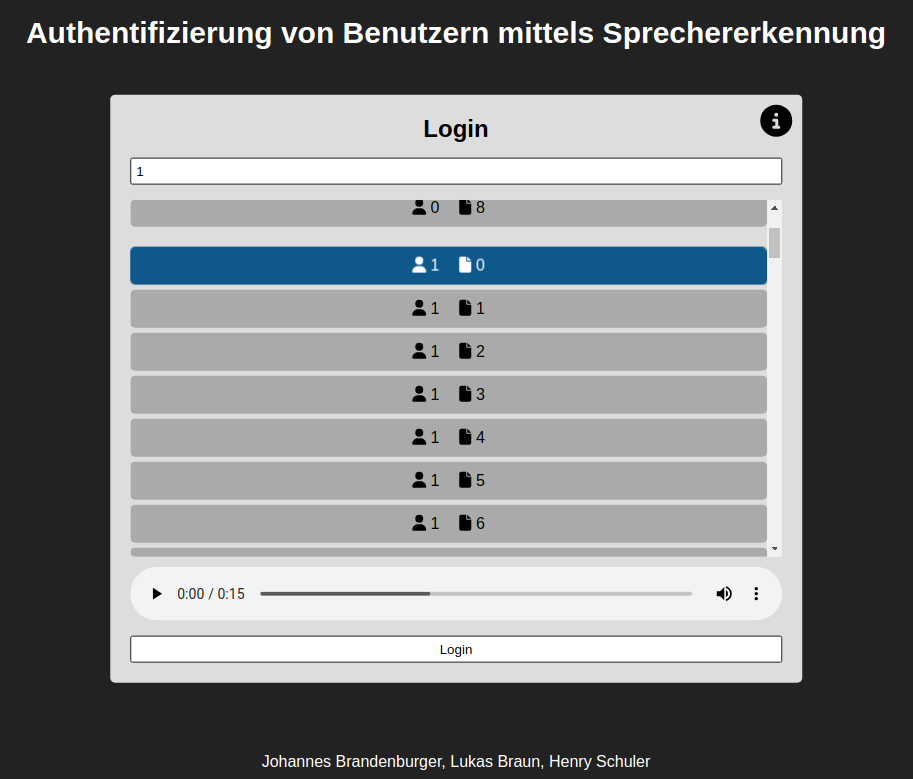
\includegraphics[width=0.9\textwidth, keepaspectratio]{images/UI.png}
        \subcaption{App/Login}
        \label{fig:AppLogin}
    \end{subfigure}
    \begin{subfigure}[c]{0.49\textwidth}
        \centering
        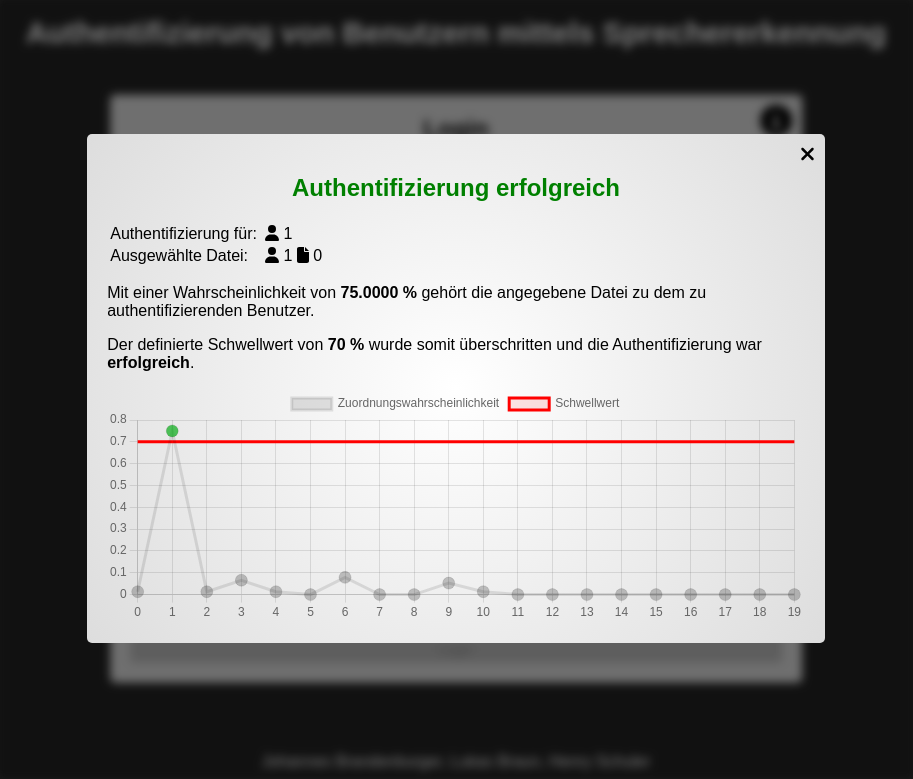
\includegraphics[width=0.9\textwidth, keepaspectratio]{images/UIResult.png}
        \caption{Result}
        \label{fig:Result}
    \end{subfigure}
    \caption{Weboberfläche}
\end{figure}
Diese unterteilt sich in zwei Abschnitte.
Zunächst kann über ein Eingabefeld die ID des zu authentifizierenden Nutzers angegeben werden.
Die Eingabe ist dabei auf die Zahlen 0-19 begrenzt.
Die Eingabe anderer Zeichen führt dazu, dass der Inhalt des Eingabefelds gelöscht wird.
Anschließend kann eine zu verwendende Audiodatei aus einer Liste ausgewählt werden.
Für die Erzeugung der Liste in der Benutzeroberfläche, wird die JSX-Funktion \textFunktion{map()} verwendet um Schaltflächen für jeweils neun Dateien pro Sprecher zu generieren (vgl. Listing~\ref{lst:AudiodateiAuswahl}, Z.~\ref{line:MapOneAppTsx},\ref{line:MapTwoAppTsx}).
Über einen \textFunktion{onClick()} Event-Listener (Z.~\ref{line:OnClickAppTsx}) wird dabei der jeweilige Index des selektierten Elements gespeichert.
\lstset{escapeinside={//(*@}{@*)}}
\begin{lstlisting}[language=HTML,caption=Auswahl der Audiodatei - App.tsx,label=lst:AudiodateiAuswahl]
<div className="fileList">
    {
        // create an array with all numbers from 0 to 20
        Array.from(Array(20).keys()).map((id) => { //(*@\label{line:MapOneAppTsx}@*)
            return Array.from(Array(9).keys()).map((fileIndex) => { //(*@\label{line:MapTwoAppTsx}@*)
                return (
                    <div 
                        key={"speaker" + id + "file" + fileIndex}
                        className={"fileItem " + (sampleFileUserId === id && sampleFileIndex === fileIndex ? "selected" : "")}
                        onClick={() => { //(*@\label{line:OnClickAppTsx}@*)
                            setSampleFileUserId(id);
                            setSampleFileIndex(fileIndex);
                        }}
                    >
                        <span>
                            <FontAwesomeIcon icon={faUser} />
                            &nbsp;{id}
                        </span>
                        <span>
                            <FontAwesomeIcon icon={faFile} />
                            &nbsp;{fileIndex}
                        </span>
                    </div>
                )
            })
        })
    }
</div>
\end{lstlisting}

Um die Benutzerfreundlichkeit zu verbessern, besteht dabei zusätzlich die Möglichkeit, die ausgewählte Datei im Browser abzuspielen.
Dafür wird (wie in Listing~\ref{lst:AudioAppTsx} dargestellt) der \ac{HTML} \textFunktion{<audio>} Tag verwendet.
Die dafür benötigten Ressourcen (WAV-Dateien) werden im Ordner \textOrdner{public/audio\_dataset} zur Verfügung gestellt.
\begin{lstlisting}[language=HTML,caption=Audio Tag - App.tsx,label=lst:AudioAppTsx]
<audio controls ref={audioRef}>
    <source src={`./audio_dataset/Speaker${String(sampleFileUserId).padStart(4, '0')}/Validation_Speaker${String(sampleFileUserId).padStart(2, '0')}_${String(sampleFileIndex).padStart(4, '0')}.wav`} type="audio/wav" />
    Audio files are not supported by your browser.
</audio>
\end{lstlisting}

Über den Login-Knopf wird die Authentifizierungsanfrage an den Server gesendet.
Der Knopf kann dabei erst durch den Benutzer gedrückt werden, wenn sowohl in dem Eingabefeld eine valide Zahl steht, als auch eine Authentifizierungsdatei ausgewählt ist.

Für die Anfrage an den Server wird die \textFunktion{fetch()} Funktion von JavaScript verwendet (vgl. Listing~\ref{lst:LoginAppTsx}, Z.~\ref{line:FetchAppTsx}).
Die zu übergebenden Parameter werden als URL-Parameter angegeben.
Ist der Server über die angegebene IP-Adresse und Port nicht erreichbar, so wird dies dem Benutzer mittels eines \textFunktion{alert()} mitgeteillt (Z.~\ref{line:AlertAppTsx}).
\begin{lstlisting}[language=JavaScript,caption=login() - App.tsx,label=lst:LoginAppTsx]
async function login(authenticatingUserId: number, sampleFileUserId: number, sampleFileIndex: number) {
    try {
        const response = await fetch(`http://${configData.SERVER_URL}:${configData.SERVER_PORT}/?speaker_id=${sampleFileUserId}&sample_id=${sampleFileIndex}&selected_speaker_id=${authenticatingUserId}`); //(*@\label{line:FetchAppTsx}@*)
    
        console.log(response)
        if (!response.ok) {
            return { 
                absolute_accuracy_of_selected_speaker: 0,
                is_authenticated: false,
                absolute_accuracy_of_all_speakers: []
            };
        }
    
        const json = await response.json();
        
        return json;
    } catch (e) {
        console.error(e);
        alert(`Es konnte keine Verbindung zum Server (${configData.SERVER_URL}:${configData.SERVER_PORT}) hergestellt werden!`) //(*@\label{line:AlertAppTsx}@*)
        return {
            absolute_accuracy_of_selected_speaker: 0,
            is_authenticated: false,
            absolute_accuracy_of_all_speakers: []
        }
    }
}
\end{lstlisting}

Die Darstellung des Ergebnisses mittels der \textKlasse{Result} Komponente ist in Abbildung~\ref{fig:Result} dargestellt.
Dem Benutzer werden sowohl seine Authentifizierungsangaben, als auch das Ergebnis der Authentifizierung in Textform angezeigt.
Die Klassifikation als \gqq{erfolgreich} oder \gqq{fehlgeschlagen} kann sowohl dem Text als auch der Farbe der Überschrift (grün oder rot) entnommen werden.

Zusätzlich erhält der Benutzer einen grafischen Einblick in die Wahrscheinlichkeitsverteilung der Zuordnung der ausgewählten Sprecherdatei zu den verschiedenen Sprechern.
Das Diagramm wird mit Hilfe der Bibliotheken chart.js und react-chartjs-2 eingebunden.

\subsubsection{Server} \label{sec:UmsetzungServer}
Wie in der Technologieentscheidung bereits erwähnt, wird der Server mithilfe der Bibliothek Flask implementiert.
Listing~\ref{lst:serverPy} zeigt dabei die wesentlichen Codeabschnitte für die Umsetzung des Servers als Flask Applikation.
\begin{lstlisting}[language=Python,caption=Ausschnitt server.py,label=lst:serverPy]
app = Flask(__name__) //(*@\label{line:FlaskAppServerPy}@*)
CORS(app)

@app.route("/", methods=["GET", "POST"])
def handle_api_request():
    ...

if __name__ == '__main__':
    app.run(debug=False, host='127.0.0.1', port=5500) //(*@\label{line:AppRunServerPy}@*)
\end{lstlisting}
Zunächst muss eine neue Flask \textVariable{app} erstellt werden (Z.~\ref{line:FlaskAppServerPy}).
Mittels \textFunktion{CORS(app)} wird dabei sichergestellt, dass eine Verbindung zwischen Client und Server trotz unterschiedlichem Ursprung möglich ist.

Die Authentifizierungsfunktion wird über die Wrapper-Funktion \textFunktion{handle\_api\_request()} und dem Decorator \textFunktion{@app.route()} als \ac{API} Endpoint verfügbar gemacht.
Die Abarbeitung der Anfragen unterteilt sich in die in Abbildung~\ref{fig:AblaufdiagrammServerHandleApiRequest} dargestellten fünf Schritte.
\begin{figure}[H]
    \centering
    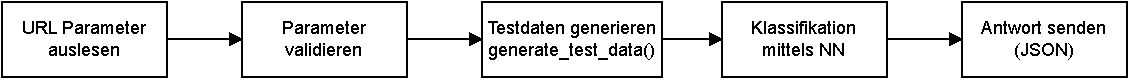
\includegraphics[width=0.9\textwidth, keepaspectratio]{images/AblaufdiagrammServerHandleApiRequest.pdf}
    \caption{Ablaufdiagramm handle\_api\_request()}
    \label{fig:AblaufdiagrammServerHandleApiRequest}
\end{figure}
Dafür werden zunächst die übergebenen Parameter aus der URL ausgelesen.
Anschließend wird überprüft ob es sich bei den Werten um numerische Werte handelt, die im vorgegebenen Definitionsbereich liegen (vgl. Listing~\ref{lst:ParameterValidationServerPy}).
\begin{lstlisting}[language=Python,caption=Parametervalidierung handle\_api\_request() - server.py,label=lst:ParameterValidationServerPy]
if not (
    speaker_id.isnumeric() and 
    sample_id.isnumeric() and 
    selected_speaker_id.isnumeric() and
    0 <= int(speaker_id) <= 19 and
    0 <= int(sample_id) <= 8 and
    0 <= int(selected_speaker_id) <= 19
):
    return parameter_error_message
\end{lstlisting}
% TODO: evtl. Ref auf genaues Kapitel aktualisieren
Da die Generierung der Testdaten analog zu Kapitel~\ref{sec:UmsetzungVersuchssystem} verläuft, wird darauf nicht weiter eingegangen.
Mit den generierten Daten wird anschließend die Klassifikation durch das \ac{NN} durchgeführt und die Ergebnisse aufbereitet und im JSON-Format an den Client zurückgesendet.

Das neuronale Netz, welches vom Server für die Authentifizierung von Benutzern verwendet wird, ergibt sich aus der Evaluation des Versuchssystems im nachfolgenden Kapitel~\ref{sec:Evaluation}.
% Hierzu wird mit der ermittelten Konfiguration ein neues neuronales Netz unter Verwendung von einer erhöhten Anzahl an Epochen generiert, um die Genauigkeit des Systems noch einmal zu verbessern.
% Vorgreifend muss hierbei erwähnt werden, dass das System durch die Erhöhung der Epochen insofern verbessert werden konnte, dass die Grenze für die Anzahl an Frames die dem zu authentifizierenden Nutzer zugeordnet werden müssen, von 65 \% auf 70 \% erhöht werden kann.
% Deshalb zeigt die Abbildung~\ref{fig:Result} in der Wahrscheinlichkeitsverteilung einen Threshold von 70 \%.

Über die Anweisung \textFunktion{app.run()} unter Angabe der IP-Adresse und des Ports, kann der Server gestartet werden (Listing~\ref{lst:serverPy}, Z.~\ref{line:AppRunServerPy}).
